% !TEX encoding = UTF-8 Unicode
% !TEX spellcheck = en-US


% This is the root file of your thesis: thesis.tex
% A line starting with % is a comment. In some cases, I have included a command preceded by a %. You may activate the command by removing the %.

%%===================================
\documentclass[12pt]{report}
\usepackage{ramsstyle}
\usepackage{parskip}
\usepackage{hyperref}
\usepackage{graphicx}
\usepackage{natbib}
%%===================================
%Write the various parts of your thesis as separate files and include them into the main file by the command \include{name of included file}. When you compile the LaTeX file, you may choose which subfiles to include by the command

%\includeonly{chapter01,chapter02}

%%===================================
\begin{document}
% !TEX encoding = UTF-8 Unicode
%!TEX root = thesis.tex
% !TEX spellcheck = en-US

%This is the Titlepage
%%=========================================
\thispagestyle{empty}
\mbox{}\\[6pc]
\begin{center}
\Huge{Crude oil inventory estimation using remote sensing}\\[2pc]

\Large{Stud.tech. Valdemar Edvard Sandal Rolfsen}\\[1pc]
\large{Desember 2017}\\[2pc]

Specialization Report\\
Department of Civil and Transport Engineering, Division of Geomatics\\
Faculty of Engineering Science and Technology \\
Norwegian University of Science and Technology
\end{center}
\vfill

\noindent Supervisor 1: Terje Midtbø

\noindent Supervisor 2: Erik Wold

 % This is the titlepage
\setcounter{page}{0}
\pagenumbering{roman}
% !TEX encoding = UTF-8 Unicode
%!TEX root = thesis.tex
% !TEX spellcheck = en-US
%%=========================================
\addcontentsline{toc}{section}{Preface}
\section*{Preface}
This report is a result of the specialization project TBA4560, at the Division of Geomatics, NTNU. The project was carried out the autumn of 2017 in cooperation with Rystad Enery, an international oil and gas knowledge house. The main supervisor has been Terje Midtbø, and Erik Wold the CTO of Rystad Energy has been the assisting supervisor.

Through the project the author has gotten a good understanding of the principles behind semantic segmentation and height estimation, and which methods that can be used to extract information from remote sensing data. Especially the field of machine learning has been very interesting to explore, because of the enormous potential that lies within its applications.

In general, the author feel that the project has provided a good insight as to how to write good and concise reports. \\[1pc]

\begin{center}
Trondheim, 2017-12-20\\[4pc]

Valdemar Edvard Sandal Rolfsen
\end{center}
% !TEX encoding = UTF-8 Unicode
%!TEX root = thesis.tex
% !TEX spellcheck = en-US
%%=========================================
\addcontentsline{toc}{section}{Acknowledgment}
\section*{Acknowledgment}
I would like to thank the following persons for their great help during \ldots

If the project has been carried out in cooperation with an external partner (e.g., a company), you should acknowledge the contribution and give thanks to the involved persons.

You should also acknowledge the contributions made by your supervisor(s). 


\begin{flushright}
O.N.\\[1pc]
VR
\end{flushright}

% !TEX encoding = UTF-8 Unicode
%!TEX root = thesis.tex
% !TEX spellcheck = en-US
%%=========================================
\addcontentsline{toc}{section}{Abstract}
\section*{Abstract}
Cushing, Oklahoma, a major crude oil trading hub, is often referred to as the famous price settlement point for West Texas Intermediate of the New York Mercantile Exchange. It lies a significant economic potential in knowing the inventory numbers of this area before they are released.

This paper investigates different approaches to estimate the total inventory using remote sensing techniques, including standard approaches for semantic segmentation, machine learning, height estimation using SAR and InSAR analysis and trigonometrical height estimation using building shadows cast by the sun.

These methods are then compared, evaluated and combined to find the approach that is most likely suitable for accurately retrieving the inventory numbers.
\tableofcontents
\setcounter{page}{0}
\pagenumbering{arabic}
% !TEX encoding = UTF-8 Unicode
%!TEX root = thesis.tex
% !TEX spellcheck = en-US
%%=========================================
\chapter{Introduction}
Segmantic segmentation and feature extraction in remote sensing, has been a field of research for many decades. The ability to extract geospatial information directly from satellite imagery has been crucial for fields such as environmental and demographic research. Furthermore, a vast development within the field of machine learning and artificial intelligence the last years, has enabled many researchers to find useful applications of such algorithms within their own scientific fields.

With new satellite technology providing frequently updated imagery, with resolutions less than 0.5 meters, the amount of data that can be extracted is almost incomprehensible. This paper focuses on how automatic height estimation of ground objects can be achieved through remote sensing, semantic image segmentation and different height estimation techniques.

The main goal of this study is to investigate different methods for automatic detection and height retrieval of the roofs of oil tanks in Cushing, Oklahoma. By knowing the height difference between the tanks floating roofs and their actual height, it is possible to calculate their inventory.

%%=========================================
\section{Background}
% In this section, you should present the problem that you are going to investigate or analyze; why this problem is of interest; what has, so far, been done to solve the problem, and which parts of the problem that remain.

Satellites has been collecting earth observation data for decades. Since the satellite Explorer 6 took the first picture of the earth in 1959, millions of satellite images has been taken, processed and stored \cite{Esa2009a}. This information however, has been very difficult to access, and even harder to analyze when accessible. However, during the last decade, the development of machine learning based methods for Earth Science applications has experiences a considerable leap forward \cite{Lary2010}.

In 2014 the first satellite in the new family of earth observation satellites, called the Sentinels, was launched from Kourou, French Guiana. Since then 7 different constellations, each consisting of two satellites,  have been launched, and are now orbiting and monitoring the earths surface. The goal of these satellites is to produce a continuous stream of timely data for Europe's Copernicus program, which will be used for environmental monitoring. The different constellations have different missions when it comes to providing datasets for the Copernicus Service. While some provide very specific data, such as monitoring the earths atmosphere, other constellations provide more general data, such as multi-spectral, high-resolution imagery of the earths surface. In order to maximize the usage of these temporal datasets, they have all been provided free of charge to the public. Other satellite constellations such as SkySat \citep{Planet2017} and WorldView \citep{DigitalGlobe2017} provide even more accurate satellite imagery, with submeter resolutions. With these satellites providing frequently updated imagery over most parts of the earths surface, the amount of earth observation data that can be observed is huge. 

This means that data that earlier required manual measurements in order to be analyzed, now can be gathered, processes and analyzed automatically at a high phase. One field where this can provide valuable information is within the oil industry.

Cushing Oklahoma is the major trading hub and famous price settlement point for West Texas Intermediate of the New York Mercantile Exchange. With inventory numbers not being continuously updated by Energy Information Administration (EIA), there exists a potential in retrieving these numbers automatically through remote sensing.

%%=========================================
\section{Problem}
%You should define your problem in a clear an unambiguous way and explain why this is a problem, why it is of interest---and to whom. It is also important to delimit the problem area.

The paper aims to answer if it is possible, with todays methods and satellite technology to automatically provide frequently updated estimations of the total inventory of all the crude oil tanks in Cushing, Oklahoma.

%%=========================================
\section{Approach}
%Here you should describe the (scientific) approach and experiments that you will use or have used to solve the problem and meet your objectives and tasks. Experiments may in this context relate analyses you need to carry out in order to investigate a specific hypothesis, task objective, or similar. You should specify the approach and experiments for each objective and/or task. It is preferred that you supplement your explanation of the approach with an illustration.

This paper will focus on investigating theory and previous work related to semantic segmentation of satellite images and techniques for height detection using data collected through remote sensing. By combining these two elements of study, it is theorized that it can be possible to automatically locate and estimate the inventory of oil tanks in Cushing, Oklahoma.

\subsection*{Semantic segmentation}
In terms of semantic segmentation the paper discuss different approaches ranging from standard methods, such as the Hough transform to newer, more advanced methods such as image segmentation using convolutional neural networks. The goal is to present the strengths and weaknesses of the different methods, in order to determine which one is most suitable to the task in hand. 

\subsection*{Height estimation}
There are also a large variety of different methods for height estimation using data from satellite imagery. While the methods investigated related to semantic segmentation only focus on multispectral images, both methods related to radar images and multispectral imaged are considered for height estimation. The methods that are investigated are SAR, InSar and shadow measurements.

%%=========================================
\section{Limitations}
%In this section you describe the limitations of your study. These may be related to the study object (physical limitations, operational limitations), to the environmental and operational conditions, to the thoroughness of the analysis, and so on.

This study is conducted as a literature review, and does not present any implementation of the methods that are investigated.

%%=========================================
\section{Outline}
%Here, you give an overview of how the remaining part of the report is organized. A proposed structure of the main chapters in the report can be as follows (note that some chapters are not numbered):
The remaining part of this paper consists of the following chapters:

\begin{itemize}
\item Chapter 2. Theoretical background: This chapter gives a theoretical background of the different methods that are investigated later in the paper. It provides the basic knowledge required in order to understand the different methods presented in related work.
\item Chapter 3. Related Work: In this chapter the previous work relevant for this paper is presented. It includes standard methods for image segmentation, an overview of the advances in convolutional neural networks and how they can be used for image segmentation. Furthermore, different works related to height estimation of buildings are presented.
\item Chapter 4. Evaluating the methods: The focus in this chapter is to evaluate and compare the different methods that have been investigated in the previous chapters.
\item Chapter 5. Conclusions, discussion, and ideas for further work: A conclusion is presented based on the previous chapters, the overall 
\item Bibliography
\end{itemize}
\chapter{Theoretical background}
%Here you identify and give the theoretical background needed in this report, with proper references to each literature reference used. The selection of what to include should be discussed and agreed with the supervisors. Theory may involve concepts, definitions, methods, regulations/key standards, theory to explain specific system behavior, and so on.
In this chapter we are going to investigate some of the key concepts related to pattern recognition, shape detection in imagery and height estimation from remote sensing. 

\section{Shape detection}
Identifying geometric shapes in computer vision has been a classical problem for decades. There are many theories related to what is the best way of detecting a particular shape in an image, with shapes defines as two dimensional features of an object that are invariant to scene factors, or whose variation can be modeled easily \citep{Moon2002}.

\subsection{The Hough transform}
In image analysis, the Hough Transform is a technique used for feature extraction. This technique uses a voting procedure from which object candidates are obtained as local maxima in a space constructed by the algorithm (called a accumulator space). Since the algorithm requires that the desired features are specified in some parametric from, the classical Hough transform is mostly used for the detection of regular curves (lines, circles ellipses, etc.).

The main idea of the algorithm is that each edge pixel contributes to a globally consistent solution, such as a curve. In order to detect a points contribution to this solution, the algorithm performs a point-to-curve transformation from the cartesian image coordinate space, to a polar Hough parameter space. In the cartesian coordinate space, a line segment can be represented by \autoref{eq:parametric}.

\begin{equation}
	xcos(\theta) + ysin(\theta) = r
	\label{eq:parametric}
\end{equation}

In \autoref{fig:parametricline} each point (x,y) on the line corresponds to a set of constant $r$ and $\theta$ values.

\begin{figure}[!h]
	\centering
	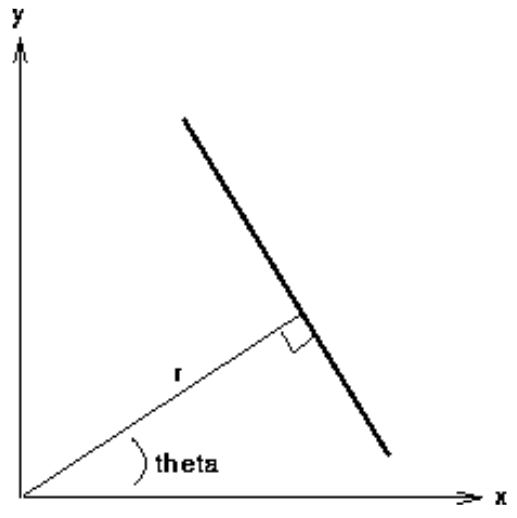
\includegraphics[scale=0.3]{fig/parametric-line.png}
	\caption{Parametric line represented by \autoref{eq:parametric} \citep{Fisher2003}}
	\label{fig:parametricline}
\end{figure}

Therefore when viewed in the Hough parameter space, points that are collinear in the cartesian space will yield curves which intersect at common $r$ and $\theta$ values. Here bright areas (high degree of intersection) indicates collinearity between points in an image.

\begin{figure}[!h]
	\centering
	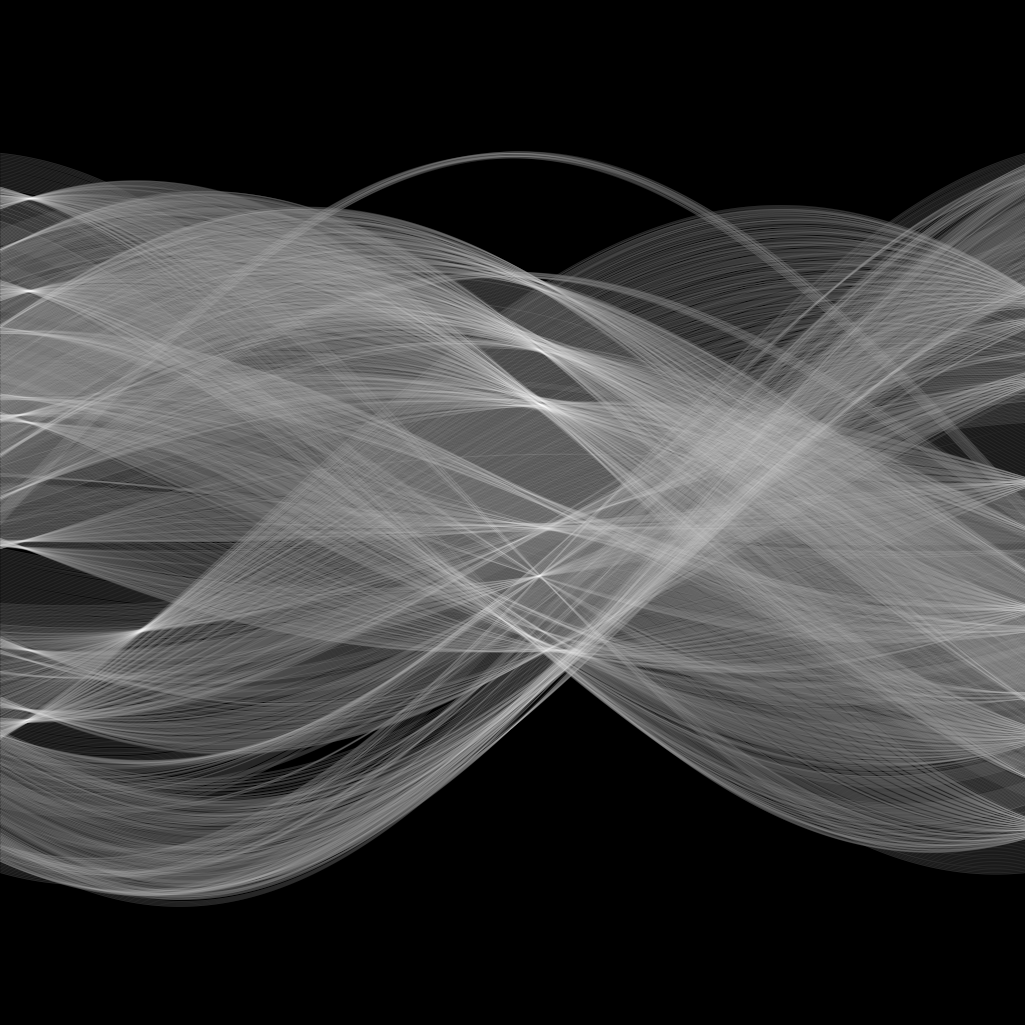
\includegraphics[scale=0.2]{fig/hough_transform.png}
	\caption{Parametric line represented by \autoref{eq:parametric} \citep{Fisher2003}}
	\label{fig:parametricline}
\end{figure}

For detecting circles the computational complexity of the algorithm increases, because the parametric equation representing a circle requires a three dimensional Hough parameter space (see \autoref{eq:parametriccircle}).

\begin{equation}
	(x-a)^{2}+(y-b)^{2} = r^{2}
	\label{eq:parametriccircle}
\end{equation}

\subsection{Shape detection using superpixels}
Most images are based on a raster format, meaning that pixels in the image are structured as an array or grid, where each pixel is associated with a position (row and column), and a numeric value. Raster images can represent a range of different shapes, where a point can be represented by a single pixel and a circle by a contiguous collection of pixels \citep{Worboys2003}. Even though rasters are easy to work with in most computer systems, since they are represented the way that they are, they do not contain any information about the topology of the objects in the image. For example, there is no way of knowing if a pixel is contained within a certain object or not. In order to identify objects, one approach is therefore to detect edge pixels.

In recent years shape detection algorithms have come to increasingly rely on superpixel algorithms, which groups pixels into perceptually meaningful atomic regions \citep{Achanta2012}. Such regions replace the regular, rigid structure of the raster grid, as shown in \autoref{fig:superpixels}.

\begin{figure}[!h]
	\centering
	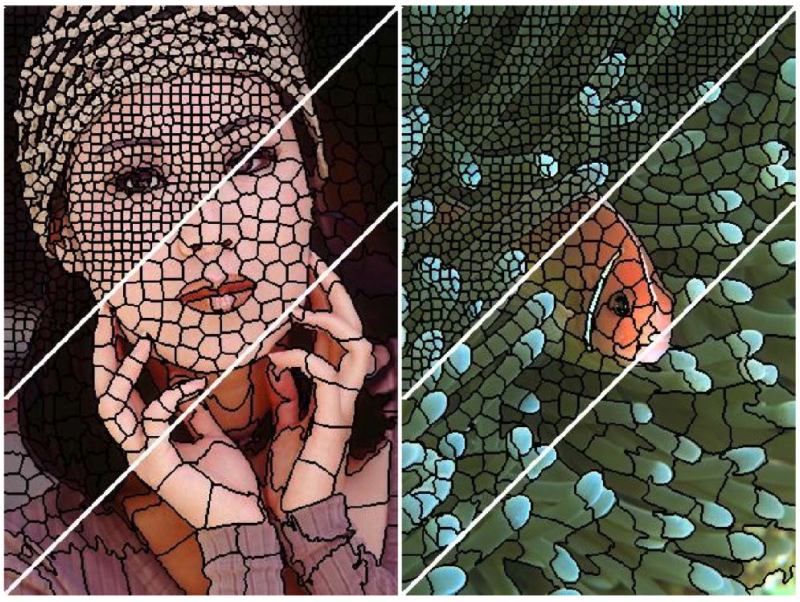
\includegraphics[scale=0.3]{fig/superpixels}
	\caption{Visualization of image segmentation using SLIC \citep{Achanta2012}}
	\label{fig:superpixels}
\end{figure}

When constructing superpixels, there are some properties of the algorithm that are desirable, regardless of the problem that are being solved. These are, according to \citep{Achanta2012}, the following three points:

\begin{itemize}
	\item Superpixels should adhere well to image boundaries
	\item When used to reduce computional complexity as a preprocessing step, superpixels should be fast to compute, memory efficient, and simple to use.
	\item When used for segmentation purposes, superpixels should both increase the speed and improve the quality of the results.
\end{itemize}

\section{Artificial Neural Networks}
In recent years, the development of machine learning, a branch of artificial intelligent systems, has become increasingly important in terms of pattern and object recognition in remote sensing and image analysis in general. One of the most commonly used approaches for data mining in remote sensing, has been artificial neural networks \cite{Lary2016}.

The basic principle behind artificial neural networks (ANNs) is that it is built up by a network of many simple units that are working in parallel with no centralized control unit. The networks primary means of storage are the weights between the individual units, and the network learns by updating these weights in relation to being provided with a training example.

In order to understand the behavior of ANNs it is important to understand their structures. The most common structure for an ANN is what is called a Feed-forward neural network structure.

\subsection{Feed-forward neural networks}
A feed-forward neural network is build up by a given number of connected layers. A layer is a collection of simple units, called artificial neurons. All networks must consist of an input and output layer, but can also contain an optional number of hidden layers. A network that only consists of an input and output layer is called a perceptron, and it has been shown that these types of networks are only able to model linear functions \citep{Minsky1969}.

\paragraph{Input Layer}
The input layer is the layer that feeds the information into the network. Here the number of neurons are typically equal to the number of features in the data.

\paragraph{Hidden layer}
The hidden layers in an ANN is what enables the network to learn and model nonlinear functions. It is the weights on the connections between the different layers that enables the network to encode the information extracted from the training data.

\paragraph{Output layer}
In order to extract the answer or prediction from the model, an output layer has to be present. Depending on the setup of the neural network, the output value can either be a real value or a set of probabilities. The output type is dependent on the activation that is chosen for the layer. What an activation function is, and how it effects the output of a layer will be discussed later in this section.

A feed forward network can either be fully og partly connected. In a fully connected network, all the neurons in each layer has a connection to all neurons in the previous layer, and all neurons in the next layer, while in a partly connected layer only some of the neurons are connected.

\subsection{Training a neural network}
The main purpose of a well trained ANN is to be able, by using its weighted connections, to amplify the signal and dampen the noise of the data it has been trained on. It does so by altering the different weights and biases in a way that allocates significance to some features and removing it from other. This way the model can learn which features are tied to which outcomes.

Neural networks learn these relationships by making a guess based on the input, weights and biases, and then get feedback on how accurate the guess was. It is the loss function related to the model, such as stochastic gradient decent (SDG), which gives this feedback by rewarding good guesses and penalizing bad ones.

The most common learning algorithm associated with neural networks is the \textit{backpropagation learning algorithm}.

\subsubsection{Backpropagation learning}
The backpropagation algorithm learns by first trying to compute a training examples output value, by taking a forward pass through the network. If the output matches the label associated with the example nothing happens, but if it does not the weights has to be updated.

In order to update the weights in the network, \autoref{eq:backupdate} is used.

\begin{equation}\label{eq:backupdate}
	W_{j,i} \Leftarrow W_{j,i}+ \alpha*a_{j}*Err_{i}*g'(input\_sum_{i})
\end{equation}

\autoref{eq:backupdate} is called the weight update rule for the connection between neuron $j$ and $i$ as seen in \autoref{fig:backpropagationtwolayers}. Furthermore, $\alpha$ is the learning rate (discussed in \autoref{section:hyperparameters}), $a_{j}$ is the incoming activation function, $Err_{i}$ is the error in $i$ and $g'(input\_sum_{i})$ is the derivative of the activation function over the input sum as seen in \autoref{eq:activation}.

\begin{equation}\label{eq:activation}
a_{j} = g(input\_sum_{j})
\end{equation}

where the input sum is given by:

\begin{equation}\label{eq:inputsum}
	input\_sum_{i} = W_{i}*A_{i}+b
\end{equation}

\begin{figure}[!h]
	\centering
	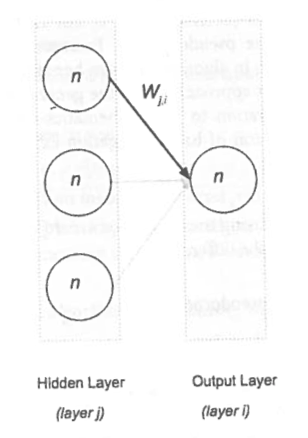
\includegraphics[scale=1]{fig/backpropagation_two_layers.png}
	\caption{The two last layers of an multilayer feed-forward neural network \cite{Patterson2017}}
	\label{fig:backpropagationtwolayers}
\end{figure}

The backpropagation algorithm traverses the network backwards, updating the weight of connection between each layer, as describd in \autoref{eq:backupdate}, until it reaches the input layer. This way the weights and biases that have been assigned the blame for the error are reduced, while the ones that supporting the correct answer are strengthened. 

\subsection{Activation functions}
Activation functions are scalar-to-scalar functions which are used to propagate the output of one layer to the next, and it is what enables the network to model nonlinear functions. This section will discuss some of the most common activation functions used in ANNs.

\paragraph{Linear}
The linear activation function, $f(x) = Wx$ is the simplest activation function and is often associated with the input layer of the network. It says that the dependent variable $x$ is proportional with the independent variable $Wx$.

\paragraph{Sigmoid}
The sigmoid activation function belongs to the class of logistic activation functions. It reduces extreme values or outliers in the example data, without removing them. One could see the sigmoid function as a machine that coverts independent variables of near infinite range into probabilities between 0 and 1.

\paragraph{Tanh (and Hard Tanh)}
Another class of activation functions are the hyperbolic trigonometric functions. The tanh function represents the ratio between the hyperbolic sine sine to the hyperbolic cosine, which means that unlike the sigmoid function, it has a normalized range between -1 and 1. The hard tanh activation function simply adds hard caps to the range, setting all values larger than 1 and smaller than -1 to respectively 1 and -1. The advantage of these functions are that they can deal more easily with negative numbers.

\paragraph{Softmax}
The softmax function, also referred to as the normalized, exponential function, is a generalization of the logistic function. Its function is that it returns the probability distribution over mutually exclusive output classes. For example, if the softmax activation function was applied to the vector [1, 2, 3, 4, 1, 2, 3], the result would be [0.024, 0.064, 0.175, 0.475, 0.024, 0.064, 0.175,]. As seen from this example, the function is most often used to weight the largest value and dampen values that are considerably smaller. 

\paragraph{ReLU}
The rectified linear unit function is currently considered the state of the art activation function. It can be described as $f(x)=max(0,x)$, meaning that it, above a certain threshold the output has a linear relationship with the dependent variable, it is else zero.

\subsection{Loss functions}
When working with artificial neural networks, we often talk about the ideal state of the network, meaning the state that classifies all the examples correctly. The loss function is a way of quantifying how close a network is to this ideal state. This is done by aggregating the errors produced by the networks prediction over the entire dataset, and average this value to get a single number that represents how close the network is to its ideal state. In other words, by minimizing the loss function, the network gets as close as possible to its ideal state, resulting in an optimization problem where the solution can be approximated well with iterative optimization algorithms.

There are different loss functions that are appropriate for regression and classification problems, however for the purpose of this project report it is only relevant to discuss the ones related to classification problems.

\paragraph{Hinge loss}
For hard classification, for example with discrete classes [sell=0, buy=1], the hinge loss function is most commonly used. It is also used by a class of models called maximum-margin classification models such as support vector machines, which are discussed in \autoref{section:svm}.

\paragraph{Logistic loss}
Often probabilities are of greater interest than hard classifications, in such situations the logistic loss function is of more value. An important remark when computing probabilities, is that all values has to be in the range 0 to 1 and that the probability of mutually exclusive outcomes should sum up to 1. Therefore, it is essential that the last layer uses the softmax activation function.

Optimizing the logistic loss function is the same as optimizing the "maximal likelihood", which means that the algorithm should maximize the probability that it predict the correct class, and do so for each single sample in the dataset. 

NOT FINISHED HERE

\subsection{Hyperparamenters}\label{section:hyperparameters}
In machine learning, hyperparameters deal with controlling the optimazation functions during learning, making sure that they neither overfit or underfit the data, but at the same time learns as quickly as possible.

\paragraph{Learning rate}
The learning rate, as seen in \autoref{eq:backupdate}, is a coefficient that scales the size of each weight update step. In other words, the learning rate decides how much of the computed gradient that should be used for each step. 

\paragraph{Regularization}
Regularization is important in order to control what is called out-of-control parameters. This is done by controlling the trade-off between finding a good fit on the training data and limiting the weight on features with high-polynomials. This is because such features tend to overfit the training examples.

\paragraph{Momentum}
Momentum is often described as the the learning rate of the learning rate. What it does is to prevent the learning algorithm from getting stuck in local minimas.

\paragraph{Sparsity}
Lastly, the sparsity hyperparameter helps recognize which features of the input examples that are relevant. This is important because in some datasets, the feature arrays for each example will be very different in terms of values.

\subsection{Convolutional neural networks}
In recent years, convolutional neural networks (CNNs) have been recognized as very suitable for object recognition in images \cite{Patterson2017}. One of the main reasons why the world, research society recognizes the power of deep learning have been the efficancy of CNNs image recognition capabilities. The name comes from the networks use of convolutions, a mathematical operation on two functions in order to produce a third.

\subsubsection{Biological Inspiration}
As all neural networks, CNNs are very inspired by the biological neurons in animal brains. The CNNs are especially inspired by the visual cortex, which cells are very sensitive to small subregions of the input. One often say that these cells act as local filters over the input space, which also is the case for CNNs.

\subsubsection{Difference from regular feed-forward multilayer neural networks}
A well known problem when it comes to analyzing image data using regular feed-forward multilayer neural networks, is that they do not scale well with increasing image sizes. Imagine an color image with the size 400x400 pixels (which would be a regular sized picture) that are used as input for a ANN. Such an image, represented as a vector, would create $400*400*3=480 000$ different weight connections for each neuron in the first hidden layer. For a fully connected network, this would be the case for all layers to come, which would create a tremendous amount of weight connections.

Convolutional neural networks solve this issue by representing the images in a three-dimensional structure, meaning that the input data is represented as a three-dimensional matrix with:

\begin{itemize}
	\item Image width in pixels
	\item Image height in pixels
	\item RGB channels in depth
\end{itemize}

As will be discussed later, this structure is how CNNs have evolved from previous feed-forward networks, in terms of computational efficiency.

\subsubsection{Architecture}
The purpose of the network is to transform the input examples through a series of connected layers, into a set of class scores. A general architecture is presented in \autoref{fig:cnnarchitecture}.

\begin{figure}[!h]
	\centering
	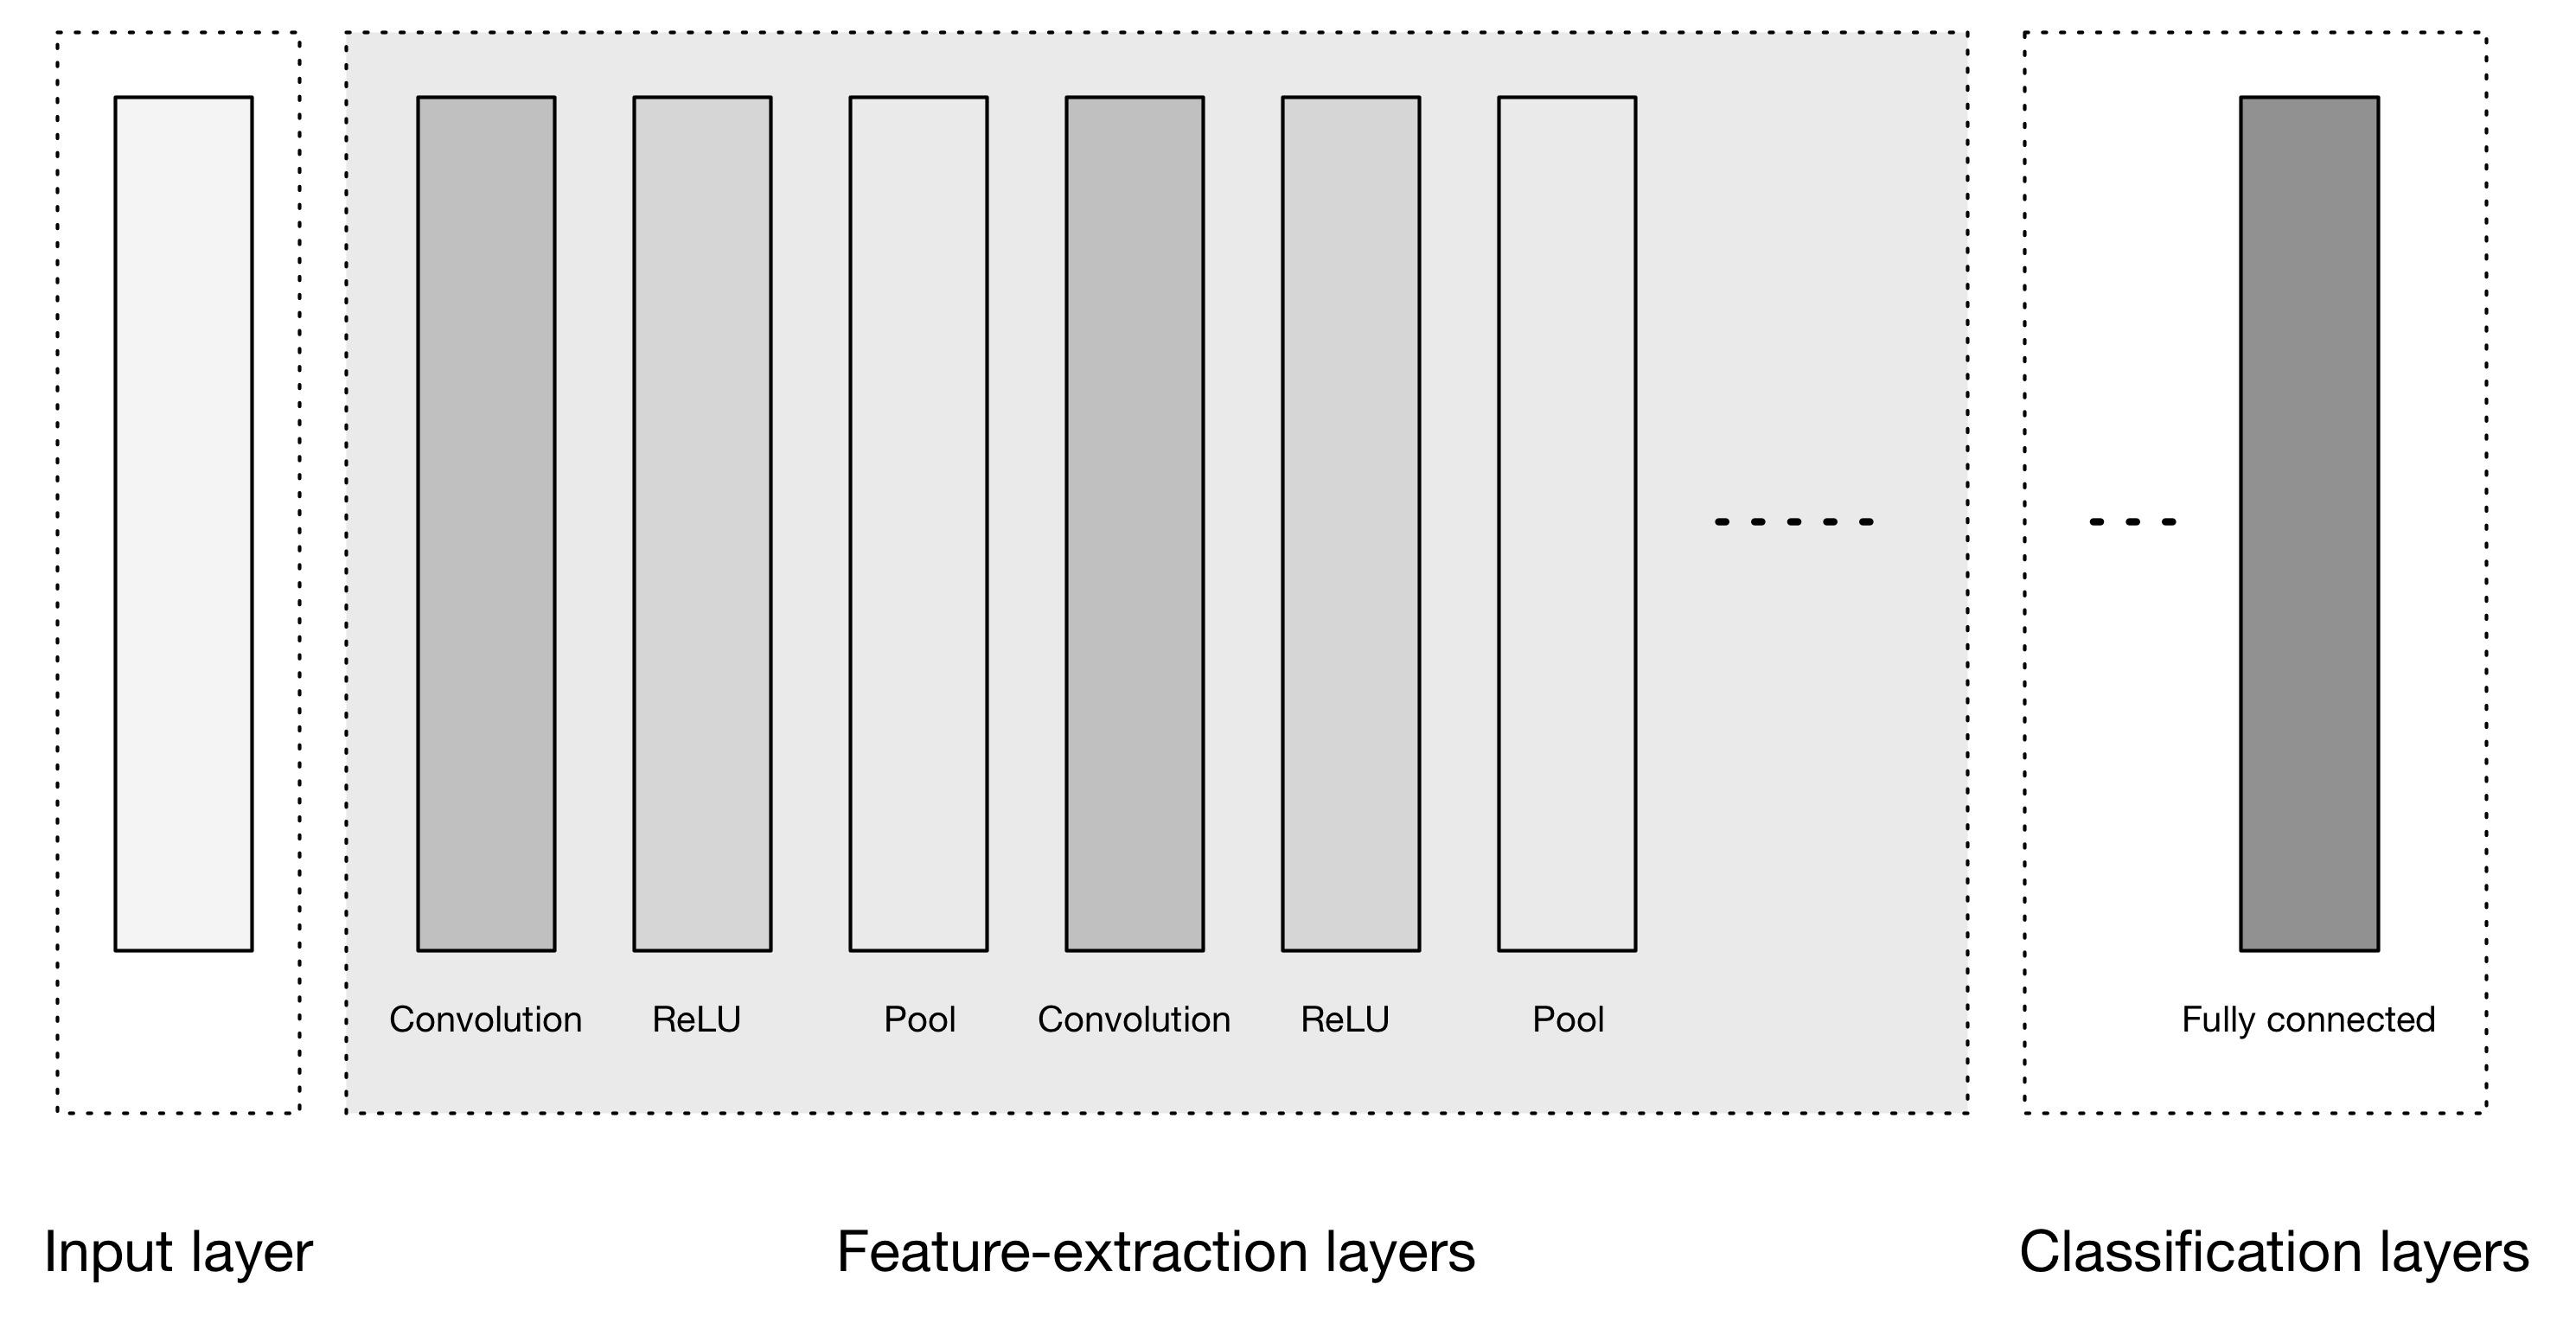
\includegraphics[scale=0.6]{fig/cnn_architecture.png}
	\caption{A general presentation of the architecture of CNNs \cite{Patterson2017}}
	\label{fig:cnnarchitecture}
\end{figure}

As seen in \autoref{fig:cnnarchitecture} the network can be divided into three sections; Input, Feature-extraction and Classification layer(s). The most interesting part of this structure is the feature-extraction layers, which is used to identify a number of features in the images, and from these construct higher-order features. The strategy of constructing high-order features is one of the key aspects of deep learning.

\remark{ It is important to note that in a CNNs layers, the neurons are arranged in a three-dimensional structure, in order to match the input data, as described earlier.}

\subsubsection{Convolutional layers}
The convolution layers, seen in \autoref{fig:cnnarchitecture}, detect features in an image through what is called the convolution operation. As mentioned in the beginning of this chapter is a convolution operation a mathematical operation that transforms two functions (or sets of information) into one, through Fourier transformations. The way that this works, is that the layer applies certain filters, called kernel filters, to segments of its input using a technique called sliding window.\footnote{A technique that slides over a set of data, only analyzing a pre-defined patch size at a time \cite{Stanford2017}} The convolution operator is described in  \autoref{eq:convop}, where $I$ is the input data and $K$ is the kernel filter of size $h*w$.

\begin{equation}\label{eq:convop}
(I*K)_{xy} = \sum_{i=1}^{h}\sum_{j=1}^{w}K_{ij} \cdot I_{x+i-1,y+j-1}
\end{equation}

Such filters can for example be an edge kernel, which only passes through information containing edges. In most cases applying a filter means reducing the size of the data, thus reducing the number of neurons in each, upcoming layer.

\begin{figure}[!h]
	\centering
	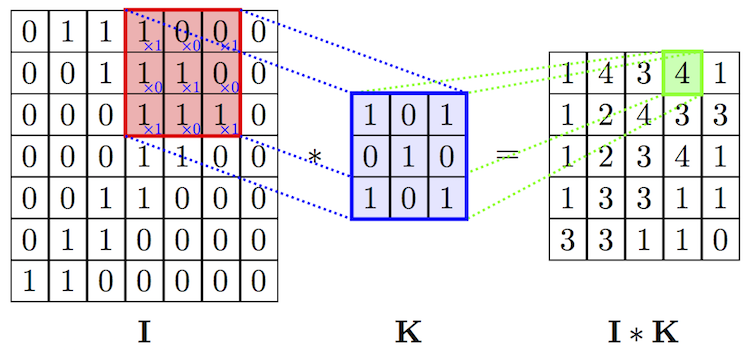
\includegraphics[scale=1.5]{fig/kernel_filter.png}
	\caption{The convolution operation (applying a kernel filter) \cite{Cambridge2017}}
	\label{fig:cnnarchitecture}
\end{figure}

\subsubsection{ReLU layers}
As seen in \autoref{fig:cnnarchitecture}, ReLU activation functions are often used in separate layers. This layer does not change the dimension of the input volume, but can change some of the pixel values.

\subsubsection{Pooling layers}\label{section:pooling}
The pooling layers is an other important part of the convolutional neural networks. They help prevent overfitting, by reducing the size of the input data using what is called max pooling, as shown in \autoref{fig:maxpooling}
\begin{figure}[!h]
	\centering
	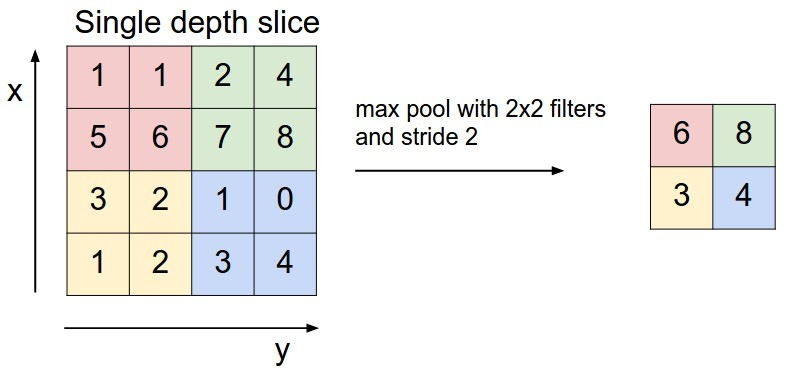
\includegraphics[scale=0.5]{fig/pooling_layer.jpeg}
	\caption{Example of max pooling operation \cite{Karpathy2017}}
	\label{fig:maxpooling}
\end{figure}

\autoref{fig:maxpooling} presents a max pool with a 2x2 filter size, and a stride of 2, meaning that 2x2 pixels are compared and that the sliding window moves 2 pixels for each comparison. I practice this means that the 75\% of the activations from the previous layer is discarded.

Links:\\
https://www.pyimagesearch.com/2014/10/20/finding-shapes-images-using-python-opencv/\\
https://www.pyimagesearch.com/2016/02/08/opencv-shape-detection/
\\
http://melvincabatuan.github.io/SLIC-Superpixels/
\\
https://www.gislounge.com/shadows-angles-measuring-object-heights-satellite-imagery/
\\

\section{Height estimation using remote sensing}\label{section:theoreticheight}

There are many different ways of estimating heights using satellite data, which involves using lidar data, SAR data and regular satellite multispectral imagery. This section will give the theoretical background for some of the most commonly used techniques.

\subsection{Synthetic Aperture Radar (SAR)}
The first technique involves using a Synthetic Aperture Radar on a moving platform, in this case a satellite. By sequentially transmitting electromagnetic waves onto the earths surface and collecting the reflected echos, the SAR satellites are able to collect high-precision, 3-dimensional data.

One of the key advantages of the SAR satellites is that they take advantage of the fact that they are moving quickly. Since the transmission and reception occurs at different times, the platform has moved, thus creating a synthetic aperture that is much larger than the satellite antenna (see \autoref{fig:syntheticaperture}).

\begin{figure}[!h]
	\centering
	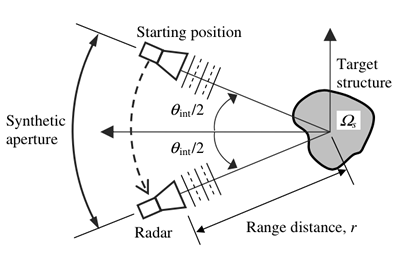
\includegraphics[scale=0.7]{fig/sar.jpg}
	\caption{Concept of syntetic aperture \cite{Yu2012}}
	\label{fig:syntheticaperture}
\end{figure}

The technique provides a finer spatial resolution to the collected data, making it possible to do height estimations with a sub-decimeter accuracy.

\subsubsection{Interferometric synthetic aperture radar (InSAR)}
While SAR makes use of amplitude and absolute phase of the returned signal, InSAR use a differential phase of the reflected signal, represented in what is called a phase image.

Looking at a phase image completely isolated will not prove very useful, as it would appear visually random. This is because in practice, the phase of the return signal is affected by a lot of different factors, resulting in no apparent correlation between the pixels in the image.

In order to get useful information these phase images, some of the factors, discussed above, has to be removed. The process of doing so is referred to as interferometry, and it uses two phase images taken from the exact same position in order to generate a interferogram (see \autoref{fig:interferogram}).

\begin{figure}[!h]
	\centering
	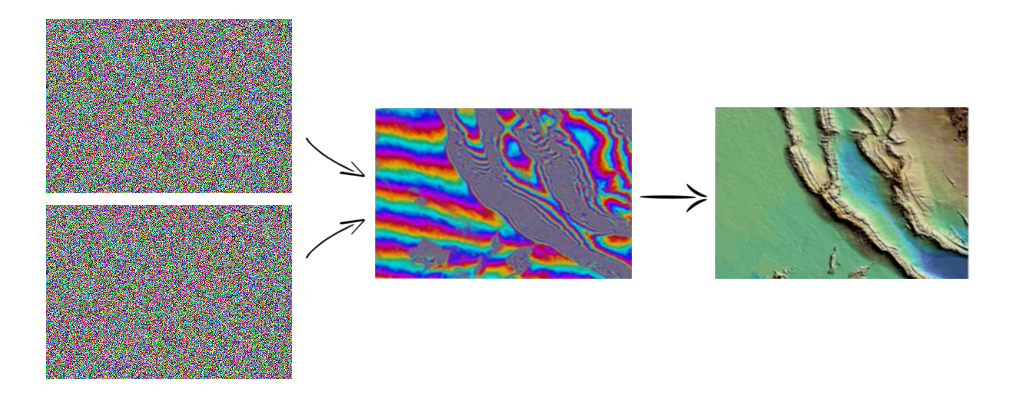
\includegraphics[scale=0.4]{fig/inferiogram.png}
	\caption{Generating an interferogram}
	\label{fig:interferogram}
\end{figure}

Producing an inferiogram consists of multiple steps:

\paragraph{Co-registration}
Using a correlation function the two images are co-registered by finding the offset and difference in geometry between them.

\paragraph{Re-sampling}
In the re-sampling step, one of the images (referred to as the slave) is re-sampled in order to match the geometry of the other (called the master). What this means in practice is that each pixel represents the same area of ground in both images.

\paragraph{Cross-multiplication and flattening}
After re-sampling the images the inferiogram is generated by taking the cross product of each pixel, and the interferometric phase due to the curvature of the earth is removed (flattening).

\paragraph{Filtering}
Lastly, it is common to filter the basic inferiogram in order to amplify the phase signal, and to interpolate over phase jumps in order to produce a continuous deformation field.

\subsection{Light Detection And Ranging (LIDAR)}
Another high precision technique for generating height data using satellites is using LIDAR. LIDAR is a surveying method that uses a pulsed ultraviolet, visible of near infrared light laser to map an area or an object. In the same way as SAR and InSAR, it used the reflected signal to measure the distance from the transmitter to the object.

\subsection{Height detection using shadows from imagery}
For height estimation of specific objects, shadow estimations can be applied. This technique uses a high resolution image, as well as knowledge about the position of the sun, the position of the image projection center and the length of the projected shadow in order to estimate an objects height (\autoref{fig:heightestimation}).

\begin{figure}[!h]
	\centering
	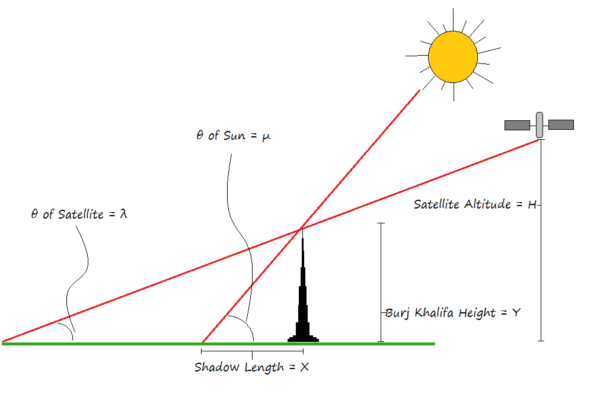
\includegraphics[scale=0.5]{fig/height_estimation.png}
	\caption{Height estimation of Burj Khalifa using shadow estimation \citep{GISLounge2014}}
	\label{fig:heightestimation}
\end{figure}

Looking at \autoref{fig:heightestimation} the height of the object can be found by:

\begin{equation}
	tan(\mu) = \frac{H_{object}}{L_{shadow}} \quad \Rightarrow \quad L_{shadow} = \frac{H_{object}}{tan(\mu)}
\end{equation}

Since the satellite image rarely is taken with the projection center directly above the object (nadir angle = 0\textdegree), the blocked length of the shadow has to be estimated. Since the height of the object is the unknown, estimating the blocked length of the shadow is an iterative process, where a new calculated, temporary value for the height is used in each iteration. Calculating the length of the blocked shadow is also very straight forward: 

\begin{equation}\label{eq:blockedshadow}
	tan(90 - \lambda) = \frac{L_{blockedshadow}}{H_{object}} \quad \Rightarrow \quad L_{blockedshadow} = H_{object}*tan(90-\lambda)
\end{equation}

In \autoref{eq:blockedshadow} 90-$\lambda$ defined as the Off-nadir angle.

It is important to remember that if this technique shall produce exact results, some parameters has to be known in the moment of the capture:

\begin{itemize}
	\item The position of the satellite
	\item The time
	\item The position of the object with the unknown height
\end{itemize}

\chapter{Related Work}

\section{Standard methods for shape detection}
Before looking at the use of neural networks for shape recognition in images, some more standard approaches are presented.

\subsection{Shape detection using the Hough Transform}
Shape detection and feature extraction in images, using Hough Transforms has been a subject of research for many years. The algorithm was first popularized in computer vision in 1981 by \cite{Ballard1981} which applied a generalized version of the algorithm to detect of curves in grayscale images.

The article describes how boundary detection plays a crucial role for feature extraction in images, and how a generalized Hough algorithm can use edge information to define a mapping from the orientation of an edge point to a reference point related to the shape.

\subsection{Simple Linear Iterative Clustering (SLIC)}
\cite{Achanta2012} proposes a superpixel-segmentation algorithm (SLIC), which in their opinion is best suited to meet these demands. They compare their algorithm to a variety of state-of-the-art superpixel methods and conclude that none of the existing techniques are satisfactory in regards to the points.

The SLIC algorithm is relatively simple to understand. One of its fundamental principles is that, by limiting the search space for each cluster center (points in the regular raster grid), it reduces the search speed significantly. This is achievable due to the fact that one of the primary goals of the algorithm is to create a set of approximately equal-sized superpixels. Thus, instead of searching the whole raster grid for each cluster center, the algorithm only has to search for edge pixels at a distance equal to D, as shown in \autoref{eq:distanceSuperpixel}.

\begin{equation}
	D'=\sqrt{\left(\frac{d_{c}}{m}\right)^{2} + \left(\frac{d_{s}}{S}\right)^{2}}
	\label{eq:distanceSuperpixel}
\end{equation}

In \autoref{eq:distanceSuperpixel} $d_{c}$ is the Euclidean distance between two pixels in terms of color and $d_{s}$ is the pixels euclidean, spatial distance. Furthermore, $S$ is the sampling interval of the cluster centers ($S = \sqrt{N/k}$, where N is the number of pixels in the grid and k is the desired number of superpixels) and $m$ is a fixed constant based on the color diversity in the image.

Since the algorithm generates superpixels by clustering pixels based on their color and spatial proximity, creating a five-dimensional, \textit{labxy} space, one would think that the distance could be found by simply taking the 5D Euclidean distance. However, it turns out that for large superpixels, spatial distance outweighs the color proximity. Which is why the two distances $d_{c}$ and $d_{s}$ are weighted.

\section{The development of Convolutional neural networks}
Since McCulloch and Pitts created what is acknowledged as the first neural network in 1943, using simple electrical circuits \citep{Mcculloch1990}, they have played an essential role in the field of pattern recognition. 

Since the late 1990's the idea of using convolutional operations in these networks has been considered more and more prominent \citep{LeC}, and this approach is still one of the leading research fields within ANN research \citep{Wu2017}. This section will discuss the development of the convolutional neural networks the last two decades.

\subsection{Early adaption of convolutional neural networks}
The earliest attempts of using convolutional operations for pattern and object recognition in neural networks was first made nearly twenty years ago by \cite{LeC}. In the paper, a convolutional neural network is used to analyze handwritten characters.

\subsection{Deep Convolutional Neural Networks}
It was, however, not until Alex Krizhevsky, Geoffrey Hinton, and Ilya Sutskever won the ImageNet \footnote{ImageNet is a very large dataset consisting of 15 million labeled, high-resolution images divided into over 22.000 categories.} 2012 competition (ILSVRC'12), that CNN's became acknowledged as one of the most sophisticated approaches for image recognition. Their deep convolutional neural network (commonly called AlexNet) consisted of five convolutional layers, each followed by a pooling layer (max-pooling), and three fully-connected softmax layers \citep{Krizhevsky2012}. The network applied two different methods; Data Augmentation and Dropout layers, to reduce overfitting.

Even though the AlexNet was a significant breakthrough for the convolutional neural networks, it was criticized for not presenting a good ground for understanding what was happening inside the network, thus making it hard to improve. One of the solutions to this problem is the ZF Net, which applies deconvolutional neural networks \citep{Zeiler2011} to map the dense feature space produced by a CNN back to its original pixel space \citep{Zeiler2014}. \autoref{fig:deconv} shown how a deconvolutional network can help visualizing the feature space of a CNN.

\begin{figure}[!h]
	\centering
	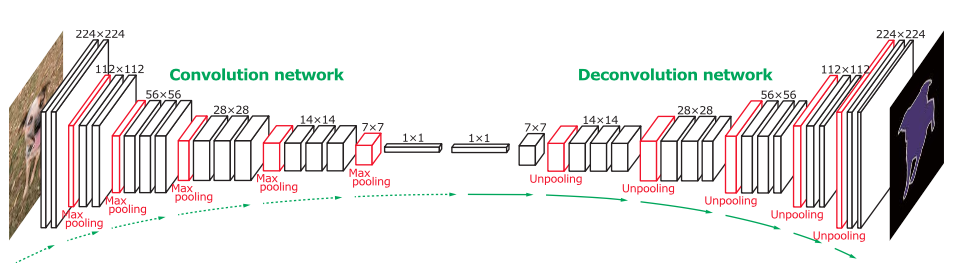
\includegraphics[scale=0.5]{fig/deconv.png}
	\caption{Process of visualizing the feature space of a CNN \citep{Noh2015}}
	\label{fig:deconv}
\end{figure}

To do so, the ZF Net successfully unpool, rectify and filter the feature map, generated by the CNN, to reconstruct the activity inside the network. 

\paragraph{Unpooling} In general, the max-pooling operation is non-reversible, since there are no tracking of the positions of the selected features, as seen in \autoref{section:pooling}. Therefore, to reconstruct the feature map, the location of each selected maxima had to be stored.

\paragraph{Rectification}
Their CNN used the common ReLU activation function for each Convolution Layer. Therefore the reconstruction layers also need to use this activation function to prevent negative values.

\paragraph{Filtering}
Since CNN's apply kernel filters to each convolution layers input volumes, the filtering has to be inverted when reconstructing. To do so, the same filters are transposed (remember that the filters are matrices) and applied to the rectified activation maps.

\subsubsection{GoogLeNet}
Another network, whose creators have criticized the standard structure of the convolutional neural networks, is the GoogLeNet \citep{Szegedy2014}. The authors of the article claim that their network was significantly more accurate than the AlexNet, while at the same time only using one-twelfth of the parameters.

The GoogLeNet introduces what is called an inception architecture (see \autoref{fig:inception} ), which the main idea is to cluster neurons in the network which have highly correlated outputs. This is because, in images, the correlation between pixels tend to be local. 

\begin{figure}[!h]
	\centering
	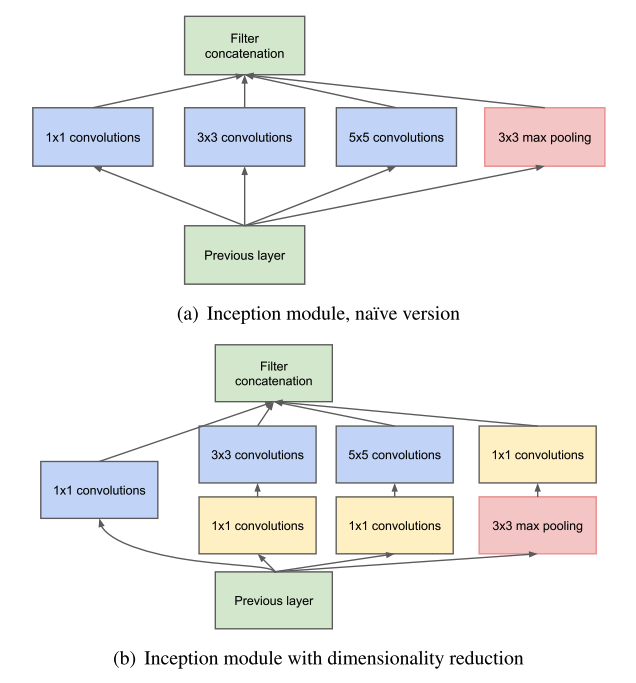
\includegraphics[scale=0.5]{fig/inception_layer.png}
	\caption{Two versions of the inception module \citep{Szegedy2014}}
	\label{fig:inception}
\end{figure}

The basic structure of the inception module is to do multiple convolution operations, in parallel, with different sized filters, and then concatenate the results before passing them on to the next layer. Additionally, a parallel pooling operation is added to each inception module, because such operations have proven them selfs successful in other CNN's.

The naive version of these "micro-networks" is shown in \autoref{fig:inception} (a). One issue with this naive version is that, even with a modest number of 5x5 convolutions, the computational cost can be quite expensive. This is solved by keeping the representation of the information as sparse as possible, and only compress the signals when they have to be aggregated. To do so, 1x1 convolutions are used to compute reductions before the 3x3 and 5x5 convolutional operations are applied (\autoref{fig:inception} (b)).

\subsubsection{VGGNet}
Another example of a successful deep convolutional neural network is the VGGNet. This network does not present any new concepts, but the authors argue that by stacking multiple layers, doing small convolutional operations (3x3 and a few 1x1) they can outperform the other discussed networks \citep{Simonyan2014}.

\begin{figure}[!h]
	\centering
	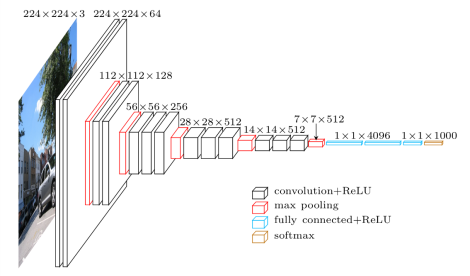
\includegraphics[scale=0.7]{fig/vgg16.png}
	\caption{The 16-layer VGGNet \citep{Frossard2016}}
	\label{fig:inception}
\end{figure}

An important difference between this network and previous networks is that the creators focus on depth, thus calling the network a very deep convolutional network.

\subsubsection{ResNet}
A problem that arises with deeper convolutional neural networks is the degradation problem. As depth increases in the network, the accuracy decreases (\autoref{fig:degradation}).

\begin{figure}[!h]
	\centering
	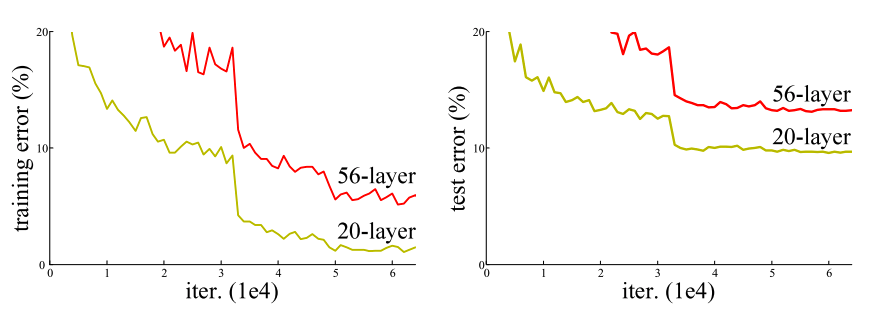
\includegraphics[scale=0.5]{fig/degradation.png}
	\caption{Degradation problem \citep{Wu2017}}
	\label{fig:degradation}
\end{figure}

Surprisingly enough this decrease in accuracy is not due to overfitting, as adding more layers effects the training error as well \citep{Wu2017}. In theory, any deep network should be able to perform at least as good as a shallower network, only by seeing the layers that differentiate the two networks as identity mappings.\footnote{The map which assigns every member of a set A to the same element  $id_{A}$. It is the same as the identity function: $id(x)=x$} This, however, does not seem to be the case in practice, suggesting that networks have problems learning identity mappings by multiple, non-linear layers.

To solve the degradation problem, the authors of the paper introduces two new concepts, which sets the foundation for their residual neural network (ResNet).

\paragraph{Residual mapping}
The paper hypothesizes that it is easier to optimize residual mapping, thus introducing the residual mapping function:

\begin{equation}
	F(x) := H(x) - x
\end{equation}

where H(x) is the desired, underlying mapping function after 2 weight layers.

\paragraph{Shortcut connections}
Connections which skip one or more layers, as seen in \autoref{fig:shortcut}, in order to obtain the desired mapping function H(x).

\begin{figure}[!h]
	\centering
	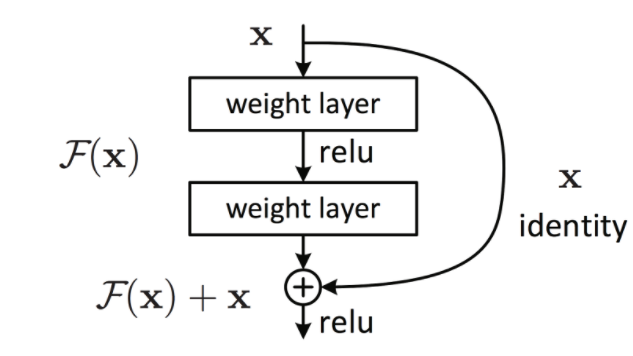
\includegraphics[scale=0.5]{fig/shortcut_connection.png}
	\caption{A residual building block \citep{Wu2017}}
	\label{fig:shortcut}
\end{figure}

Using these concepts, the authors were able to create the winning 152-layer deep ResNet of the ILSVRC'15.

\section{Semantic segmentation using convolution neural networks}
In later years there has been significant progress in the field of edge detection in imagery has been made due to advances in deep learning \citep{Yu2017}. \cite{Marmanis2016} present an end-to-end semantic segmentation method for segmentation in aerial images of the ISPRS semantic labeling dataset \footnote{Link: http://www2.isprs.org/commissions/comm3/wg4/semantic-labeling.html}. Using a Fully Convolutional Network and Conditional Random Fields, they can do a per-pixel semantic segmentation of a very high-resolution aerial image with an accuracy of 88.5\% based on five different classes.

Furthermore, \cite{Kaiser2017} present a solution, which deals with the lack of labeled training data available. To do so, the authors make use of the open-source map data library OpenStreetMap, to automatically derive weakly labeled training data. By matching this data with aerial imagery from Google Maps, and training a fully convolutional neural network, they are able to classify buildings and roads at a high level of accuracy (see \autoref{fig:aerialsegmentation}).

\begin{figure}[!h]
	\centering
	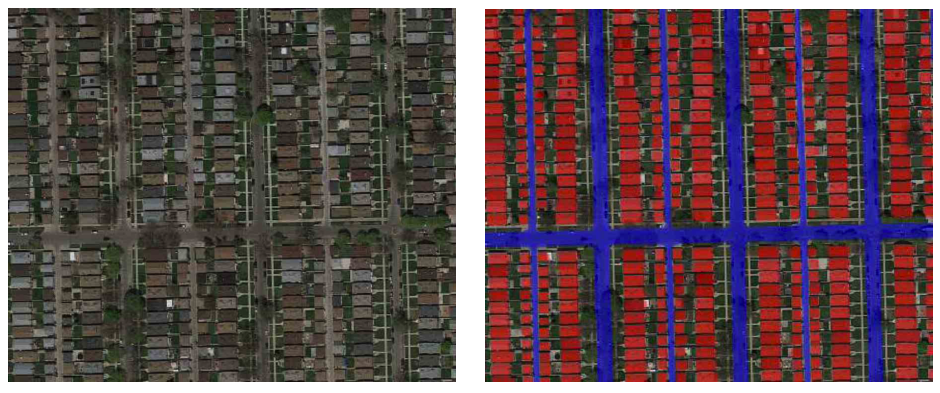
\includegraphics[scale=0.4]{fig/aerial_segmentation.png}
	\caption{Results from classification of buildings and roads \citep{Kaiser2017}}
	\label{fig:aerialsegmentation}
\end{figure}

Other attempts for semantic segmentation in remote sensing have been made with different variants of deep convolutional neural networks \citep{Kemker2017}. In their paper, they propose an approach for using the Digital Imaging and Remote Sensing Image Generation (DIRSIG) modeling software to generate a large quantity of synthetic multispectral imagery and corresponding labels. For the semantic segmentation, the authors adapt two fully-convolutional neural networks called SharpMask \citep{Pinheiro2016} and RefineNet \citep{Lin2016}. Their results show that it is possible to use synthetic imagery to assist the training of semantic segmentation networks when there is not enough annotated image data.

\section{Height estimation form a nadir perspective}
As seen in \autoref{section:theoreticheight} there are many different techniques that can be applied to estimate the height of a building. This section will focus on different attempts to retrieve height data, using satellite imagery.

\subsection{Building height retrieval from VHR SAR Imagery}
After the launch of TerraSAR-X in 2007, a satellite that was designed to acquire high-resolution X-band radar images of the entire planet, it was possible to gather SAR data with a resolution of down to 1 meter \citep{Airbus2017}. In contrast to other optical, spaceborne sensors, such as Ikonos, Quickbird, and WorldView, satellites using SAR overcome the difficulties of weather conditions and lack of sun illumination.

Using the SAR images provided by the satellite \cite{Brunner2008} was able to estimate the height of man-made structures with a sub-meter precision by automatically reconstruct 3-D models, using a "hypothesis generation-rendering-matching" procedure. The basic principle was that using an optimization algorithm, the height of a building is found by testing different height hypothesis against a single SAR image. The estimation is done without modeling its exact radiometry since this would require extensive apriori knowledge about the roughness parameters and dielectric constants of the surfaces. Generating this height model becomes an optimization problem \autoref{eq:optimizationproblem}.

\begin{equation}
	\hat{h} = arg \underset{h,\overrightarrow{s}}{max}\left\{M\left[\hat{X}_{\overrightarrow{s}}(\overrightarrow{H}),X\right]\right\}
	\label{eq:optimizationproblem}
\end{equation}

In \autoref{eq:optimizationproblem} X is the true SAR image, $\hat{X}$ is the simulated SAR image at height h, M is the matching function, and $\overrightarrow{H}$ is the simulated hypothesis.

\cite{Brunner2008} tested their method on different types of buildings, where flat buildings gave a mean accuracy of $0.3 \pm 2.1 m$. 

\subsection{Height estimation from InSAR analysis}
Another approach for height detection using SAR satellites, is interferometric SAR (InSAR) analysis, as attempted by \cite{Liu2015}. In their paper, they used images taken on December 5 and 27, 2007 to generate an interferogram over San Francisco. The technique was based on extracting potential layover areas from the interferogram and use these areas to measure the height of the buildings using the relationship between the height of an object and the layover observed in the interferogram (\autoref{eq:layoverheight}).

\begin{equation}
	\Delta\Phi=\frac{4 \pi B_{N}}{\lambda H sin{\theta}}\Delta R
	\label{eq:layoverheight}
\end{equation}

In \autoref{eq:layoverheight} $\Delta\Phi$ is the phase difference within one pixel in the layover area, $B_{N}$ is the perpendicular baseline distance, $\lambda$ is the radar wavelength, H is the satellite altitude, and $\theta$ is the angle of incidence (see \autoref{fig:insar}).

\begin{figure}[!h]
	\centering
	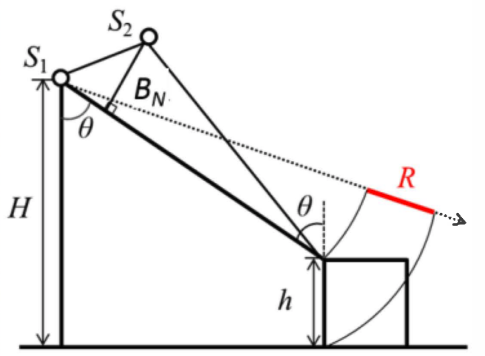
\includegraphics[scale=0.4]{fig/insar.png}
	\caption{A schematic image of geometrical characteristics for a building in a slant-range SAR image \citep{Liu2015}}
	\label{fig:insar}
\end{figure}

Using this method \cite{Liu2015} were able to estimate the height of high-rise buildings in a crowded area with a RMS of 13m and an average difference between detected results and the reference values of 6.6m.

\subsection{Height estimation using shadow measurement}
While some height extraction methods require precise specifications regarding the geometrical properties of remotely sensed data, \cite{Comber2012} present a method for determining height using building shadows. By classifying buildings and their associated shadows based on a series of different measures (see \autoref{fig:shadowclassification}), and applying \autoref{eq:shadowheight} the authors were able to give relative good height estimations.

\begin{figure}[!h]
	\centering
	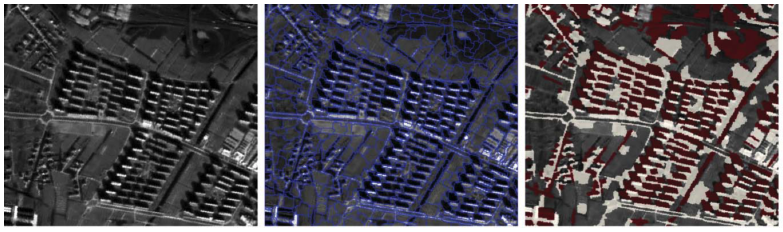
\includegraphics[scale=0.6]{fig/shadow_classification.png}
	\caption{Classification of buildings and their assiciated shadows \citep{Comber2012}}
	\label{fig:shadowclassification}
\end{figure}

\begin{equation}
	H=\frac{W}{\frac{cos(\phi_{sun}+90+\phi_{az})}{tan(\phi_{sun})}}
	\label{eq:shadowheight}
\end{equation}

Other attempts have also been made regarding estimation heights using shadows, such as \cite{Shao2011} who addresses the issue of distinguishing between shadows and water in aerial photographs. In their approach, they merged the two classes into a single shadow/water class and used different spatial indices such as object size, shape, and spatial neighbor information to separate shadow and water. They further used a standard trigonometrical approach to estimate the building heights. Their results can be seen in \autoref{fig:shadowheightresults}.

\begin{figure}[!h]
	\centering
	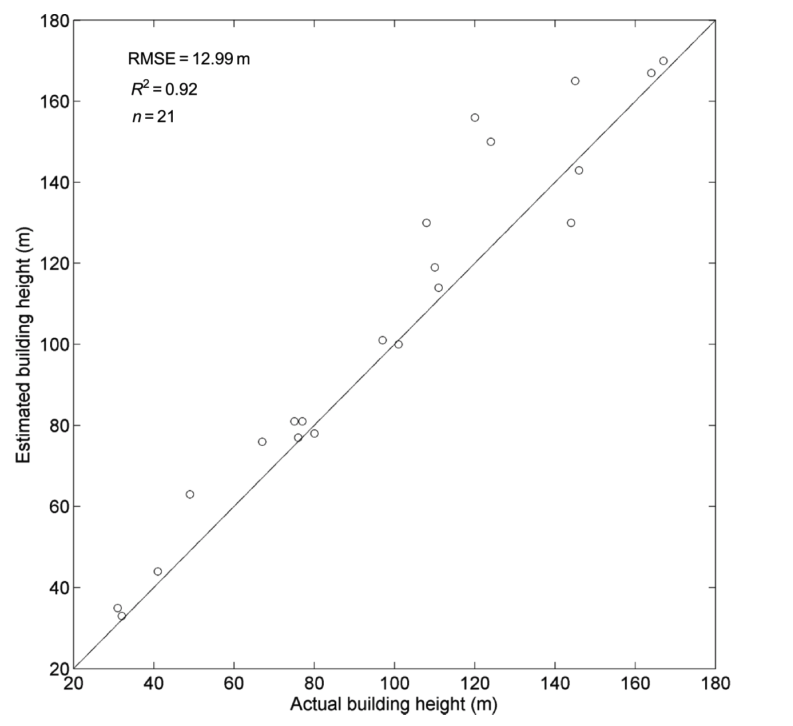
\includegraphics[scale=0.4]{fig/shadow_height_results.png}
	\caption{Accuracy evaluation of building height estimation \citep{Shao2011}}
	\label{fig:shadowheightresults}
\end{figure}
% !TEX encoding = UTF-8 Unicode
%!TEX root = thesis.tex
% !TEX spellcheck = en-US
%%=========================================
\chapter[Equations, etc]{Equations, Figures, and Tables}
The content of Chapter 2 will vary with the topic of your thesis. This chapter only gives guidance to some technical aspects of \LaTeX.
 
\begin{remark}
If you want a shorter chapter or section title to appear in the Table of Contents and in the headings of the chapter, you just include the short title in square brackets before the title of the chapter/section. Example: \begin{verbatim}\section[Short Title]{Long Title}\end{verbatim}.
\end{remark}

%%=========================================
\section{Simple Equations}
Mathematical symbols and equations can written in the text as $\lambda$, $F(t)$, or even $F(t)=\int_0^t \exp(-\lambda x)\,dx$, or as displayed equations
\begin{equation}
F(t)=\int_0^t \exp(-\lambda x)\,dx
\label{eq1}
\end{equation}


The displayed equations are automatically given equation numbers -- here (\ref{eq1}) since this is the first equation in Chapter 2. Note that you can refer to the equation by referring to the ``label'' you specified as part of the equation environment.

You can also include equations without numbers:
\begin{equation*}
F(t)=\sum_{i=1}^n \binom{n}{i}\sin(i\cdot t)
\end{equation*}

%%=========================================
\subsection*{More Advanced Formulas}
Long formulas that cannot fit into a single line can be written by using the environment \texttt{align} as
\begin{align}
F(t)&= \sum_{i=1}^n \sin(t^{n-1}) - \sum_{i=1}^n \binom{n}{i}\sin(i\cdot t) \\
      & + \int_0^\infty n^{-x} e^{-\lambda x^t}\,dt
\end{align}

In some cases, you need to write ordinary letters inside the equations. You should then use the commands 
\begin{verbatim}
\textrm  and/or \mathrm
\end{verbatim}
The first command returns the normal text font and will be scaled automatically, while the second command will be scaled according to the use.
\begin{equation*}
\textrm{MTTF}= \int_0^\infty R_\mathrm{avg}(t)\,dt
\end{equation*}



Please consult the \LaTeX\ documentation for further details about mathematics in \LaTeX.
%%=========================================
\section*{Definitions}
If you want to include a definition of a term/concept in the text, I have made the following macro (see in \texttt{ramsstyle.sty}):
\begin{defin}
\textbf{Reliability}: The ability of an item to perform a required function under stated environmental and operational conditions and for a stated period of time.\newline
\end{defin}
When text is following directly after the definition, it may sometimes be necessary to end the definition text by the command
\begin{verbatim}
\newline
\end{verbatim}
I have not included this in the definition of the \texttt{defin} environment to avoid too much space when there is not a text-block following the definition.
%%=========================================
\section{Including Figures}
If you use pdf\LaTeX\ (as recommended), all the figures must be in pdf, png, or jpg format. We recommend you to use the pdf format.  Please place the figure files in the directory \textbf{fig}. Figures are included by the command shown for Figure~\ref{fig1}. Please notice the ``path'' to the figure file written by a \emph{forward} slash (/). You should not include the format of the figure file (pdg, png, or jpg) -- just write the ``name'' of the figure. 
\begin{figure}
\centering

\includegraphics[scale=0.6,angle=15]{fig/NTNU}
\caption{This is the logo of NTNU (rotated 15 degrees).}
\label{fig1}
\end{figure}

Each figure should include a unique \emph{label} as shown in the command for Figure~\ref{fig1}. You can then refer to the figure by the \emph{ref} command.
Notice that you can scale the size of the figure by the option \texttt{scale=k}. You may also define a specific width or height of the figure by replacing the \texttt{scale} options by \texttt{width=k} or \texttt{height=k}. The factor \texttt{k} can here be specified in mm, cm, pc, and many other length measures. You may also give \texttt{k} as a fraction of the width of the text or of the height of the text, for example, \texttt{width=0.45$\backslash$textwidth}. If you later change the margins of the text, the figure width will change accordingly. As illustrated in Figure~\ref{fig1}, you may also rotate the figure -- and also do many other things (please check the documentation of the package \texttt{graphicx} -- it is available on your computer, or you may find it on the Internet).

In \LaTeX\ all figures are floating objects and will normally be placed at the top of a page. This is the standard option in all scientific reports. If you insist on placing the figure exactly where you declare the figure, you may include the command \texttt{[h]} (here) immediately after $\backslash$\texttt{begin\{figure\}}. If you will force the figure to be located either at the top or bottom of the page, you may alternatively use  \texttt{[t]} or \texttt{[b]}. For more options, check the documentation.

Large figures may be included as a \emph{sidewaysfigure} as shown in Figure~\ref{fig2}:\footnote{You can use a similar command for large tables.}
\begin{sidewaysfigure}
\centering

\includegraphics[scale=1.8]{fig/NTNU}
\caption{This is the logo of NTNU.}
\label{fig2}
\end{sidewaysfigure}

%%=========================================
\section{Including Tables}
\LaTeX\ has a lot of different options to include tables. Only one of them is illustrated here.

\begin{table}
	\centering\small
	\caption{The degree of newness of technology.}
	\label{tab1}
		\begin{tabular*}{\textwidth}{@{\extracolsep{\fill}}lccc}
			\toprule
			  &\multicolumn{3}{c}{Level of technology maturity}\\
  \cmidrule{2-4}
			Experience with the		   &  & Limited field history or not & New or \\
              operating  condition  & Proven &  used by company/user & unproven \\
        
			\midrule
			  Previous experience & 1 & 2 & 3 \\
		          No experience by company/user & 2 & 3 & 4 \\
		          No industry experience & 3 & 4 & 4 \\
			\bottomrule
		\end{tabular*}
\end{table}

\begin{remark}
Notice that figure captions (Figure text) shall be located \emph{below} the figure -- and that the caption of tables shall be \emph{above} the table. This is done by placing the $\backslash$\texttt{caption} command beneath the command $\backslash$\texttt{includegraphics} for figures, and above the command $\backslash$\texttt{begin\{tabular*\}} for tables.
\end{remark}
%%=========================================
\section{Copying Figures and Tables}
In some cases, it may be relevant to include figures and tables from from other publications in your report. This can be a direct copy or that you retype the table or redraw the figure. In both cases, you should include a reference to the source in the figure or table caption. The caption might then be written as: \textsl{Figure/Table xx: The caption text is coming here \citep{rausand04}.}

In other cases, you get the idea from a figure or table in a publication, but modify the figure/table to fit your purpose. If the change is significant, your caption should have the following format: \textsl{Figure/Table xx: The caption text is coming here \citep[adapted from][]{rausand04}.}

%%=========================================
\section{References to Figures and Tables}
Remember that all figures and tables shall be referred to and explained/discussed in the text. If a figure/table is not referred to in the text, it shall be deleted from the report.
%%=========================================
\section{A Word About Font-encoding}
When you press a button (or a combination of buttons) on your keyboard, this is represented in your computer according to the \emph{font-encoding} that has been set up. A wide range of font-encodings are available and it may be difficult to choose the ``best'' one. In the template, I have set up a font-encoding called UTF-8 which is a modern and very comprehensive encoding and is expected to be the standard encoding in the future. Before you start using this template, you should open the Preferences ->Editor dialogue in TeXworks (or TeXShop if you use a Mac) and check that encoding UTF-8 has been specified. 

If you use only numbers and letters used in standard English text, it is not very important which encoding you are using, but if you write the Norwegian letters æ, ø, å and accented letters, such as é and ä, you may run into problems if you use different encodings. Please be careful if you cut and paste text from other word-processors or editors into your \LaTeX\ file!

\subsubsection*{Warning}
If you (accidentally) open your file in another editor and this editor is set up with another font-encoding, your non-standard letters will likely come out wrong. If you do this, and detect the error, be sure \emph{not} to save your file in this editor!!

This is not a specific \LaTeX\ problem. You will run into the same problem with all editors and word-processors -- and it is of special importance if you use computers with different platforms (Windows, OSX, Linux).

%%=========================================
\section{Plagiarism}
Plagiarism is defined as ``use, without giving reasonable and appropriate credit to or acknowledging the author or source, of another person's original work, whether such work is made up of code, formulas, ideas, language, research, strategies, writing or other form'', and is a very serious issue in all academic work. You should adhere to the following rules:
\begin{itemize}
\item Give proper references to all the sources you are using as a basis for your work. The references should be give to the original work and not to newer sources that mention the original sources.
\item You may copy paragraphs up to 50 words when you include a proper reference. In doing so, you should place the copied text in inverted commas (i.e., ``Copied text follows \ldots''). Another option is to write the copied text as a quotation, for example:
\begin{quote}
Birnbaum's measure of reliability importance of component $i$ at time $t$ is equal to the probability that the system is in such a state at time $t$ that component $i$ is critical for the system.\newline \mbox{} \hfill \citet{rausand04}
\end{quote}
\end{itemize}




% !TEX encoding = UTF-8 Unicode
%!TEX root = thesis.tex
% !TEX spellcheck = en-US
%%=========================================
\chapter[Conclusions]{Conclusions, Discussion, and Recommendations for Further Work}
%%This is the last chapter
In this final chapter you should sum up what you have done and which results you have got. You should also discuss your findings, and give recommendations for further work.

%%=========================================
\section{Summary and Conclusions}
Here, you present a brief summary of your work and list the main results you have got. You should give comments to each of the objectives in Chapter 1 and state whether or not you have met the objective. If you have not met the objective, you should explain why (e.g., data not available, too difficult).

This section is similar to the Summary and Conclusions in the beginning of your report, but more detailed---referring to the the various sections in the report.

%%=========================================
\section{Discussion}
Here, you may discuss your findings based on your results, their strengths and limitations. Note that this discussion is more high level than discussions made in relation to results you have achieved and presented in the previous chapter. The discussion here should put your work in larger context. You may address if you achieved what you had intended to do, why not (if you did not), if you got results in which you did not expect, why the results are important, why there are limitations in using the results, or if there are opportunities to transfer your results and findings into other domains, and so on.
%%=========================================
\section{Recommendations for Further Work}
You should give recommendations to possible extensions to your work. The recommendations should be as specific as possible, preferably with an objective and an indication of a possible approach.

The recommendations may be classified as:
\begin{itemize}
\item Short-term
\item Medium-term
\item Long-term
\end{itemize}
% Include more chapters as required.
%%=========================================
\appendix
% !TEX encoding = UTF-8 Unicode
%!TEX root = thesis.tex
% !TEX spellcheck = en-US
%%=========================================

\chapter{Acronyms}
\begin{description}
\item[FTA] Fault tree analysis
\item[MTTF] Mean time to failure
\item[RAMS] Reliability, availability, maintainability, and safety
\end{description}
% !TEX encoding = UTF-8 Unicode
%!TEX root = thesis.tex
% !TEX spellcheck = en-US
%%=========================================

\chapter{What to put in appendixes}
This is an example of an Appendix. You can write an Appendix in the same way as a chapter, with sections, subsections, and so on. An appendix may include list of code (in case you are programming), more details about results that you have presented in the report (could be a more complete  description of results, in case you decided to focus on the most important ones in the main report), supplementary information and descriptions you have found relating to the system you are analysing, such as drawings. You may discuss with your supervisor what are relevant information for appendixes.

%%=========================================
\section{Introduction}

%%=========================================
\subsection{More Details}
% Include more appendices as required.
%%=========================================
\bibliographystyle{apa}
\addcontentsline{toc}{chapter}{\bibname}
\bibliography{bib/prosjekt}  
%%=========================================
%% !TEX encoding = UTF-8 Unicode
%!TEX root = thesis.tex
% !TEX spellcheck = en-US

%This is the Curriculum Vitae
%%=========================================
\addcontentsline{toc}{chapter}{Curriculum Vitae}
\chapter*{Curriculum Vitae}
\hrule
\begin{minipage}[t]{0.65\linewidth}
\begin{tabular}{ll}
Name: & \textbf{Your Name}\\
Gender: & Female\\
Date of birth: & 1. January 1995\\
Address: & Nordre gate 1, N--7005 Trondheim \\
Home address: & King's road 1, 4590 Vladivostok, Senegal\\
Nationality:    & English \\
Email (1): & your.name@stud.ntnu.no\\
Email (2): & yourname@gmail.com\\
Telephone: & +47 12345678\\
\end{tabular} 
\end{minipage}\hfill
\begin{minipage}[t]{0.25\linewidth}
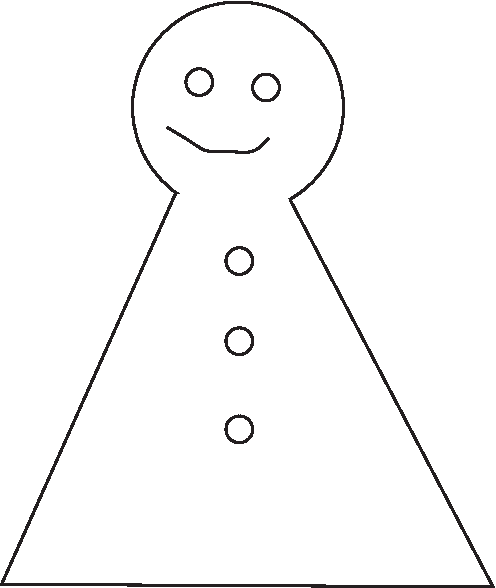
\includegraphics[scale=0.3]{fig/me}\\[1pc] Your picture
\end{minipage}
\hrule

%%=========================================
\section*{Language Skills}
Describe which languages you speak and/or write. Specify your skills in each language.

%%=========================================
\section*{Education}
\begin{itemize}
\item School 1
\item School 2
\item School 3
\end{itemize}

%%=========================================
\section*{Computer Skills}
\begin{itemize}
\item Program 1
\item Program 2
\item Program 3
\end{itemize}

%%=========================================
\section*{Experience}
\begin{itemize}
\item Job 1
\item Job 2
\item Job 3
\end{itemize}

%%=========================================
\section*{Hobbies and Other Activities}         % Your curriculum Vitae     
%%=============================================

\end{document}
